\section{Subgradients}
\frame{\tableofcontents[currentsection, hideothersubsections]}

\begin{frame}
\frametitle{Subgradients: Intro}

WHAT:\\
apply GD to \textbf{non}differentiable convex function
\vspace{5mm}

HOW:\\
use subgradient of $f(\mathbf{w})$ at $\mathbf{w}^{(t)}$, instead of the gradient;\\
(the analysis of the convergence rate remains unchanged)

\end{frame}

\begin{frame}
\frametitle{Subgradients: Intro}

\begin{figure}
    \centering
    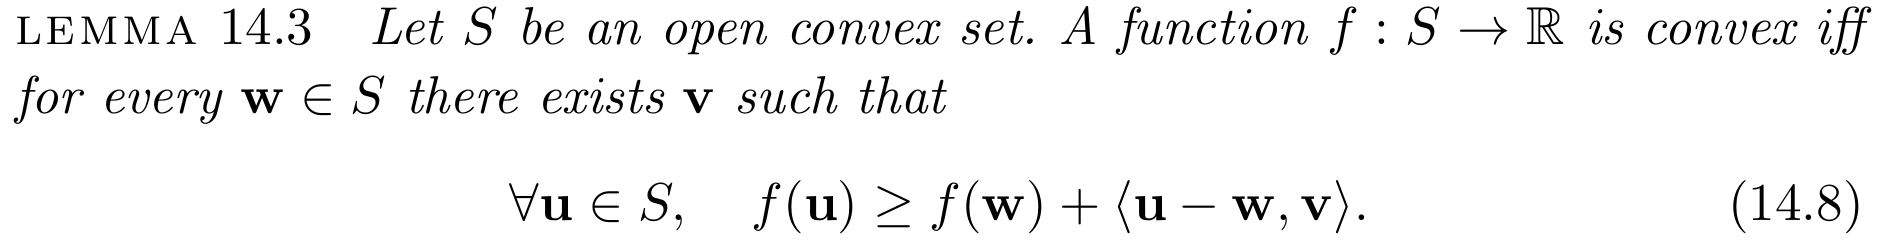
\includegraphics[scale=0.225]{lemma_14_3}
\end{figure}

\noindent\makebox[\linewidth]{\rule{\paperwidth}{0.4pt}}

\begin{figure}
    \centering
    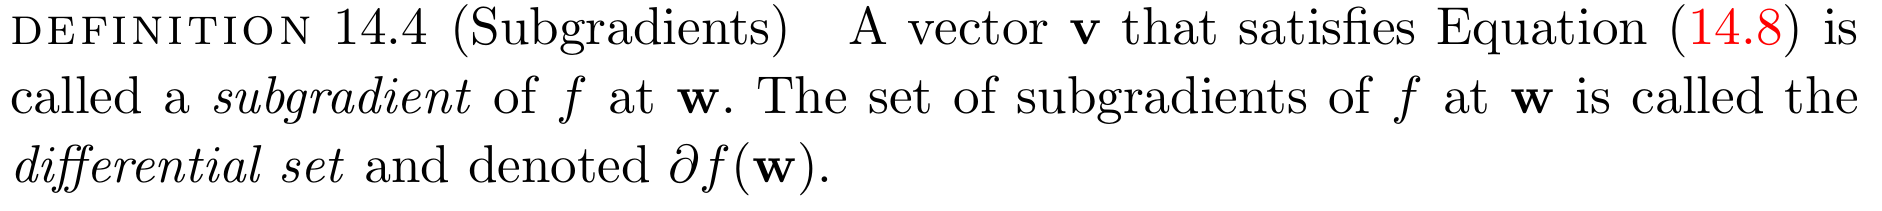
\includegraphics[scale=0.225]{def_14_4}
\end{figure}

\end{frame}

\begin{frame}
\frametitle{Subgradients: Intro}

\begin{figure}
    \centering
    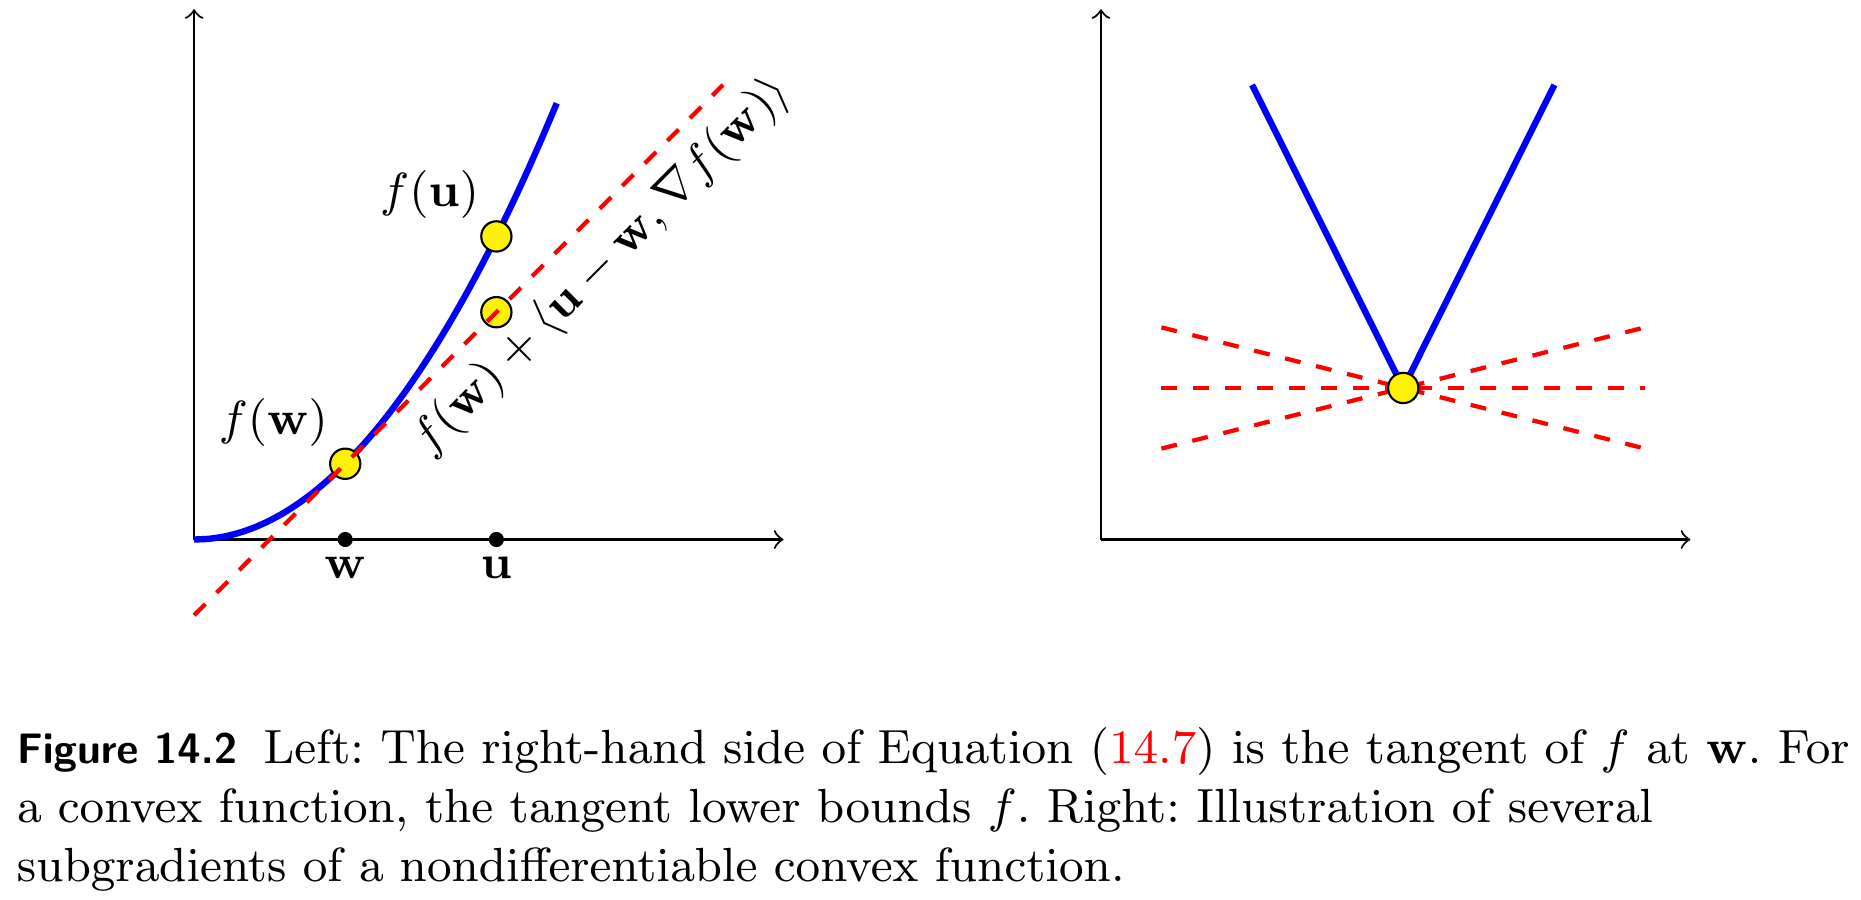
\includegraphics[scale=0.25]{fig_14_2}
\end{figure}

\end{frame}

\begin{frame}
\frametitle{Subgradients: Calculating Subgradients}

How do we construct subgradients of a given convex function?
\vspace{5mm}

For pointwise maximum functions:
\begin{figure}
    \centering
    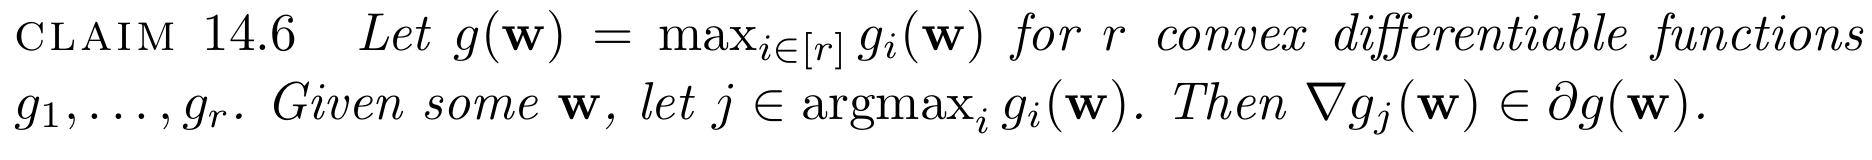
\includegraphics[scale=0.225]{claim_14_6}
\end{figure}

\begin{figure}
    \centering
    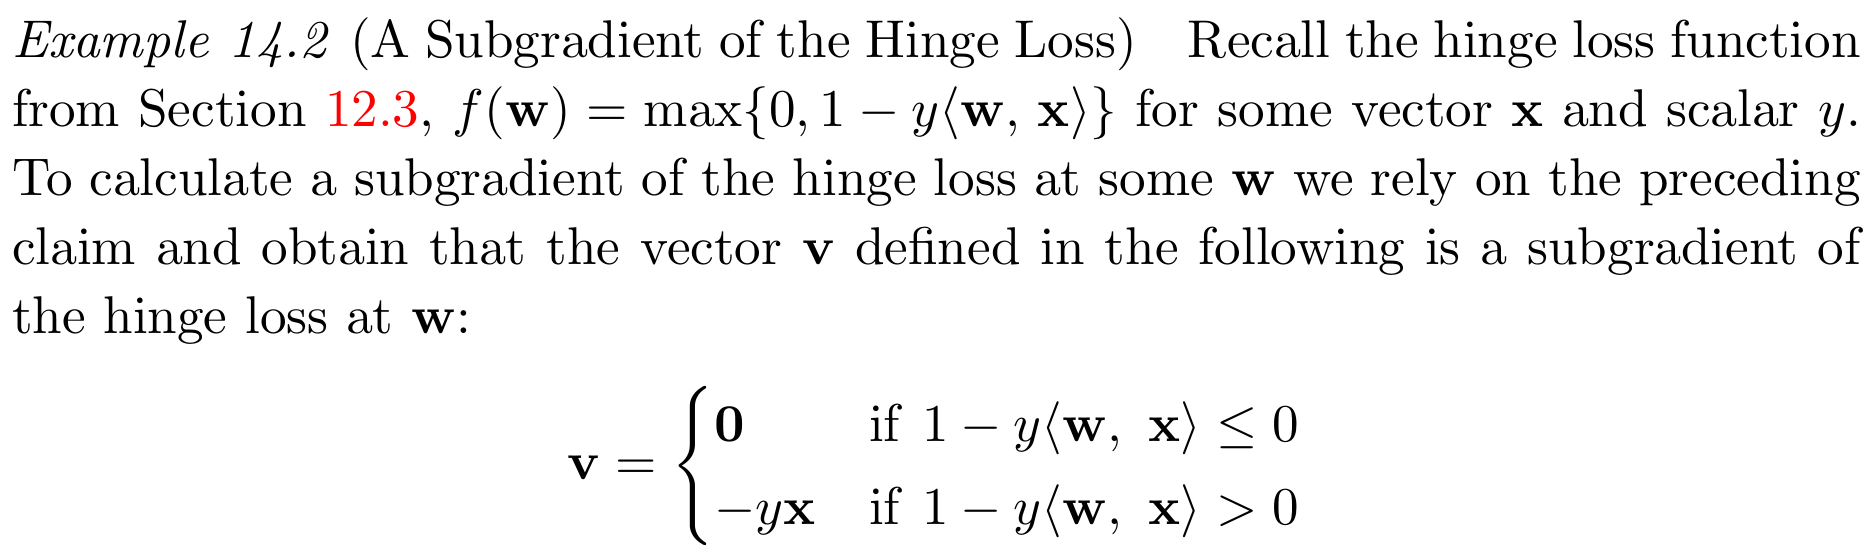
\includegraphics[scale=0.225]{example_14_2}
\end{figure}

\end{frame}
